\documentclass[oneside, class=book, 12pt, crop=false]{standalone}

\usepackage{../dissertationstyle}
\usepackage{tikz}
\usetikzlibrary{positioning}
\usetikzlibrary{shapes.geometric}
\makeatletter
\tikzset{
    database/.style={
        path picture={
            \draw (0, 1.5*\database@segmentheight) circle [x radius=\database@radius,y radius=\database@aspectratio*\database@radius];
            \draw (-\database@radius, 0.5*\database@segmentheight) arc [start angle=180,end angle=360,x radius=\database@radius, y radius=\database@aspectratio*\database@radius];
            \draw (-\database@radius,-0.5*\database@segmentheight) arc [start angle=180,end angle=360,x radius=\database@radius, y radius=\database@aspectratio*\database@radius];
            \draw (-\database@radius,1.5*\database@segmentheight) -- ++(0,-3*\database@segmentheight) arc [start angle=180,end angle=360,x radius=\database@radius, y radius=\database@aspectratio*\database@radius] -- ++(0,3*\database@segmentheight);
        },
        minimum width=2*\database@radius + \pgflinewidth,
        minimum height=3*\database@segmentheight + 2*\database@aspectratio*\database@radius + \pgflinewidth,
    },
    database segment height/.store in=\database@segmentheight,
    database radius/.store in=\database@radius,
    database aspect ratio/.store in=\database@aspectratio,
    database segment height=0.1cm,
    database radius=0.25cm,
    database aspect ratio=0.35,
}
\makeatother

\bibliography{../personal}

\begin{document}

\ifstandalone
  \graphicspath{ {./images/} }
  \setcounter{chapter}{2}
  \chapter{Implementation}
\fi
\resetfigpath{implementation}

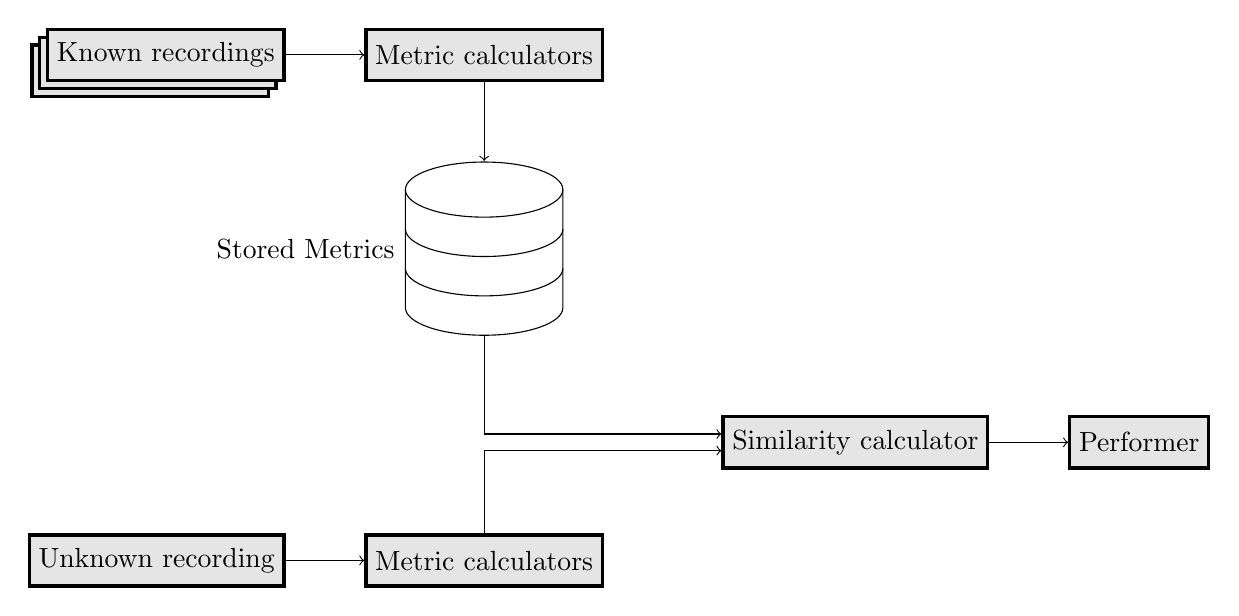
\begin{tikzpicture}[
squarednode/.style={rectangle, draw=black!100, fill=black!10, very thick, minimum size=6.5mm},
]
%Nodes
\foreach \x in {2.0, 2.1, 2.2}\node[squarednode] at (\x, \x) (knownrecordings) {Known recordings};
\node[squarednode]      (metriccalculators1)       [right= of knownrecordings] {Metric calculators};
\node[database, label=left:Stored Metrics, database radius=1cm, database segment height=0.5cm]         (storedmetrics)            [below=of metriccalculators1] {};
\node[squarednode]      (metriccalculators2) [below= 2.5cm of storedmetrics] {Metric calculators};
\node[squarednode]      (unknownrecording)  [left= of metriccalculators2] {Unknown recording};
\node[squarednode]      (similaritycalculator) [below right= 1cm and 2cm of storedmetrics] {Similarity calculator};
\node[squarednode]       (performer) [right= of similaritycalculator] {Performer};

%Lines
\draw[->] (knownrecordings.east) -- (metriccalculators1.west);
\draw[->] (metriccalculators1.south) -- (storedmetrics.north);
\draw[->] (unknownrecording.east)  -- (metriccalculators2.west);
\draw[->] (storedmetrics.south) |- ([yshift=3pt]similaritycalculator.west);
\draw[->] (metriccalculators2.north) |- ([yshift=-3pt]similaritycalculator.west);
\draw[->] (similaritycalculator.east) -- (performer.west);

\end{tikzpicture}

\ifstandalone
  \printbibliography
\fi
    
\end{document}
